\documentclass{article}

\usepackage{fancyhdr}
\usepackage{extramarks}
\usepackage{amsmath}
\usepackage{amsthm}
\usepackage{amssymb}
\usepackage{amsfonts}
\usepackage{tikz}
\usepackage[plain]{algorithm}
\usepackage{algpseudocode}
\usepackage{float} 

\usetikzlibrary{automata,positioning}

%
% Basic Document Settings
%

\topmargin=-0.45in
\evensidemargin=0in
\oddsidemargin=0in
\textwidth=6.5in
\textheight=9.0in
\headsep=0.25in

\linespread{1.1}

\pagestyle{fancy}
\lhead{\hmwkAuthorName}
\chead{\hmwkClass\ \hmwkTitle}
%\chead{\hmwkClass\ (\hmwkClassInstructor\ \hmwkClassTime): \hmwkTitle}
\rhead{\firstxmark}
\lfoot{\lastxmark}
\cfoot{\thepage}

\renewcommand\headrulewidth{0.4pt}
\renewcommand\footrulewidth{0.4pt}

\setlength\parindent{0pt}

%
% Create Problem Sections
%

\newcommand{\enterProblemHeader}[1]{
    \nobreak\extramarks{}{Problem \arabic{#1} continued on next page\ldots}\nobreak{}
    \nobreak\extramarks{Problem \arabic{#1} (continued)}{Problem \arabic{#1} continued on next page\ldots}\nobreak{}
}

\newcommand{\exitProblemHeader}[1]{
    \nobreak\extramarks{Problem \arabic{#1} (continued)}{Problem \arabic{#1} continued on next page\ldots}\nobreak{}
    \stepcounter{#1}
    \nobreak\extramarks{Problem \arabic{#1}}{}\nobreak{}
}

\setcounter{secnumdepth}{0}
\newcounter{partCounter}
\newcounter{homeworkProblemCounter}
\setcounter{homeworkProblemCounter}{1}
\nobreak\extramarks{Problem \arabic{homeworkProblemCounter}}{}\nobreak{}

%
% Homework Problem Environment
%
% This environment takes an optional argument. When given, it will adjust the
% problem counter. This is useful for when the problems given for your
% assignment aren't sequential. See the last 3 problems of this template for an
% example.
%
\newenvironment{homeworkProblem}[1][-1]{
    \ifnum#1>0
        \setcounter{homeworkProblemCounter}{#1}
    \fi
    \section{Problem \arabic{homeworkProblemCounter}}
    \setcounter{partCounter}{1}
    \enterProblemHeader{homeworkProblemCounter}
}{
    \exitProblemHeader{homeworkProblemCounter}
}

%
% Homework Details
%   - Title
%   - Due date
%   - Class
%   - Section/Time
%   - Instructor
%   - Author
%

\newcommand{\hmwkTitle}{Homework\ \#1}
\newcommand{\hmwkDueDate}{January 25, 2022}
\newcommand{\hmwkClass}{EECS 545 Machine Learning}
\newcommand{\hmwkClassTime}{Section A}
\newcommand{\hmwkClassInstructor}{Professor Honglak Lee}
\newcommand{\hmwkAuthorName}{\textbf{Yuang Huang}}
\newcommand{\hmwkUninameName}{\textbf{yahuang@umich.edu}}

%
% Title Page
%

\title{
    \vspace{2in}
    \textmd{\textbf{\hmwkClass:\ \hmwkTitle}}\\
    \normalsize\vspace{0.1in}\small{Due\ on\ \hmwkDueDate\ at 12pm}\\
    \vspace{0.1in}\large{\textit{\hmwkClassInstructor\ \hmwkClassTime}}
    \vspace{3in}
}

\author{\hmwkAuthorName\\
\hmwkUninameName}
\date{}

\renewcommand{\part}[1]{\textbf{\large Part \Alph{partCounter}}\stepcounter{partCounter}\\}

%
% Various Helper Commands
%

% Useful for algorithms
\newcommand{\alg}[1]{\textsc{\bfseries \footnotesize #1}}

% For derivatives
\newcommand{\deriv}[1]{\frac{\mathrm{d}}{\mathrm{d}x} (#1)}

% For partial derivatives
\newcommand{\pderiv}[2]{\frac{\partial}{\partial #1} (#2)}

% Integral dx
\newcommand{\dx}{\mathrm{d}x}

% Alias for the Solution section header
\newcommand{\solution}{\textbf{\large Solution}}

% Probability commands: Expectation, Variance, Covariance, Bias
\newcommand{\E}{\mathrm{E}}
\newcommand{\Var}{\mathrm{Var}}
\newcommand{\Cov}{\mathrm{Cov}}
\newcommand{\Bias}{\mathrm{Bias}}

\begin{document}

\maketitle

\pagebreak

\begin{homeworkProblem}
    \large Linear regression on a polynomial
    \\

    \textbf{Solution}
    
    %\begin{enumerate}
    %    \item \(f(n) = n^2 + n + 1\), \(g(n) = 2n^3\)
    %    \item \(f(n) = n\sqrt{n} + n^2\), \(g(n) = n^2\)
    %    \item \(f(n) = n^2 - n + 1\), \(g(n) = n^2 / 2\)
    %\end{enumerate}
    %We solve each solution algebraically to determine a possible constant
    %\(c\).
    %\\

    \textbf{Part a(\romannumeral1):} Find the coefficiets 

    \textbf{$\bullet$ Batch gradient descent(BGD)}
    
    $\qquad$Learning Rate: 0.05

    $\qquad$Epoch number: 200

    $\qquad$Degree: 1

    $\qquad$Coefficents: $\omega_0 = 1.947$, $\omega_1 = -2.824$ in the function $h(\mathbf{x}, \mathbf{w}) = \omega_0\phi_0(\mathbf{x}) + \omega_1\phi_1(\mathbf{x})$

    $\qquad$Initial value of the coefficients: Generated by taking random values from $\mathcal{N}~(0,1)$, we choose $\omega_0 = -1.376$, $\omega_1 = -1.468$


    \textbf{$\bullet$ Stochastic gradient descent(SGD)}
    
    $\qquad$Learning Rate: 0.05

    $\qquad$Epoch number: 200

    $\qquad$Degree: 1

    $\qquad$Coefficents: $\omega_0 = 1.921$, $\omega_1 = -2.853$ in the function $h(\mathbf{x}, \mathbf{w}) = \omega_0\phi_0(\mathbf{x}) + \omega_1\phi_1(\mathbf{x})$

    $\qquad$Initial value of the coefficients: Generated by taking random values from $\mathcal{N}~(0,1)$, we choose the same as the batch gradient descent where $\omega_0 = -1.376$, $\omega_1 = -1.468$\\

    \textbf{Part a(\romannumeral2):} Over-fitting

    \begin{figure}[H]  
    \centering  
    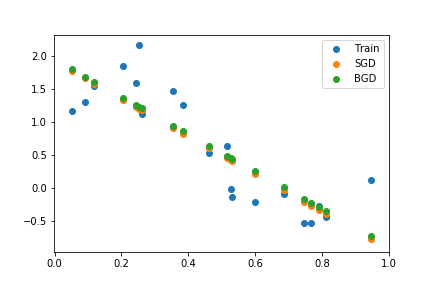
\includegraphics[width=4in,height=3.2in]{fitting_BGD_SGD.png} 
    \caption{Fitting linear regression} 
    \label{Fig1}
    \end{figure}


    \begin{figure}[H]  
    \centering  
    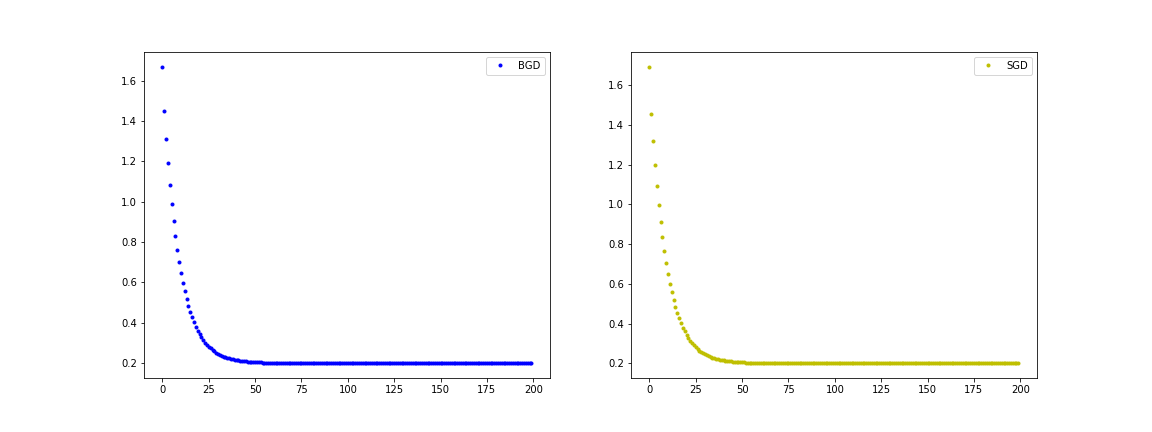
\includegraphics[width=7in,height=2.4in]{Cost_BGD_SGD.png} 
    \caption{$E_{MS}$ of BGD and SGD} 
    \label{Fig2}
    \end{figure}

    Fig. \ref{Fig1}  illustrates training data(blue), the prediction points using the BGD(green) and the SGD(orange), respectively. It is known from the figure that the fit of both methods is good and close. Fig. \ref{Fig2}  illustrates the mean squared error ($E_{MS}$) curves of the BGD and the SGD. The convergence speed of the two methods is very close (so I draw the curves separately), and they both converge at around $epoch = 50$, and converge to $E_{MS} = 0.2$. In theory, the SGD will converge faster. In problem1, it may be hard to distinguish the convergence speed of the two methods because the training set is too small.\\ \\
    \textbf{Part b(\romannumeral1):}

    \begin{figure}[H]  
    \centering  
    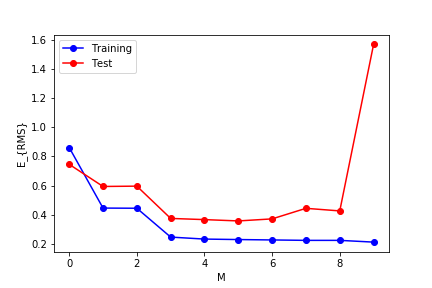
\includegraphics[width=4in,height=3.2in]{overfitting.png} 
    \caption{The trend of $E_{RMS}$ changing with degree} 
    \label{Fig3}
    \end{figure}
    \textbf{Part b(\romannumeral2):}

    Fig. \ref{Fig3} illustrates the trend of $E_{RMS}$ changing with degree. It is easy to know from the figure that 0, 1, 2, 3 degree polynomials under-fitting the date and 9 degree polynomial over-fitting the data. I think 5 degree best fits the date because  the Root-Mean-Square Error ($E_{RMS}$) of 5 degree polynomial function is relatively smaller and it needs relatively less calculations.\\ 

    \textbf{Part c(\romannumeral1):}\\
    $\qquad$The closed form solution of the ridge regression is:
    \begin{equation}
    W_{ML} = (\mathbf{\Phi^T\Phi} + \lambda\mathbf{I})^{-1}\mathbf{\Phi^Ty}
    \label{eq1}
    \end{equation}

    \begin{figure}[H]  
    \centering  
    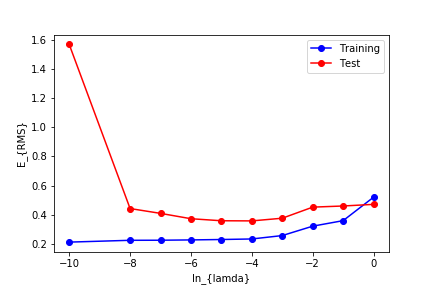
\includegraphics[width=4in,height=3.2in]{regu.png} 
    \caption{The trend of $E_{RMS}$ changing with regulization factor $\lambda$ using closed form solution} 
    \label{Fig4}
    \end{figure}

    \textbf{Part c(\romannumeral2):}\\
    As shown in Fig. \ref{Fig4}, the closed form solution reaches the lowest test $E_{RMS}$ at $\lambda = 10^{-4}$, so $\lambda = 10^{-4}$ seemed to work the best.\\

\end{homeworkProblem}

\pagebreak

\begin{homeworkProblem}
    \large Locally weighted linear regression\\

    \textbf{Solution}

    \textbf{Part 2(a):}\\
    \begin{equation}
    \begin{aligned}
    E_D(\mathbf{w}) &=(\mathbf{Xw - y})^T\mathbf{R}(\mathbf{Xw - y})
    \\
    &= \sum_{i=1}^{N}  \sum_{j=0}^{M-1} R_{ij}(\mathbf{x^{(i)}}w_j - y^{(i)})^2
    \\
    &= \sum_{i=1}^{N}R_{ij}(y^{(i)}-\mathbf{w}^{T}\mathbf{x}^{(i)})^{2}
    \end{aligned}
    \label{eq2}
    \end{equation}
    where $R_{ij}$ is the element of matrix R and 
    \begin{equation}
    R_{ij}=\left\{
    \begin{array}{ll} 
    \frac{1}{2}r^{(i)}, &i = j \\
    0, &i \neq j 
    \end{array}
    \right.
    \label{eq3}
    \end{equation}

    \textbf{Part 2(b):}\\
    Expand what we got in part2(a), we will get 
    \begin{equation}
    \begin{aligned}
    E_D(\mathbf{w}) &= (\mathbf{Xw - y})^T\mathbf{R}(\mathbf{Xw - y})
    \\
    &= \mathbf{w^TX^TRXw} - \mathbf{y^TRXw} - \mathbf{w^TX^TRy} + \mathbf{y^TRy}
    \\
    &= \mathbf{w^TX^TRXw} - 2\mathbf{w^TX^TRy} + \mathbf{y^TRy},
    \end{aligned}
    \label{eq4}
    \end{equation}
    so the gradient of $E_D(\mathbf{w})$ is shown by:
    \begin{equation}
    \begin{aligned}
    \nabla_{\mathbf{w}}  E_D(\mathbf{w}) &= \mathbf{X^TRXw} - \mathbf{X^TRy}
    \\
    &= 0 
    \end{aligned}
    \label{eq5}
    \end{equation}
    and the closed form solution is descrided by:
    \begin{equation}
    \begin{aligned}
    \Rightarrow
    \mathbf{w} &= (\mathbf{X^TRX})^{-1}\mathbf{X^TRy}
    \end{aligned}
    \label{eq6}
    \end{equation}
    
    \textbf{Part 2(c):}\\
    \begin{equation}
    P(\mathbf{Y}|\mathbf{x}^{(i)};\mathbf{w})=\prod^{N}_{i=1}\frac{1}{\sqrt{2\pi}\sigma^{(i)}}exp\left(-\frac{(y^{(i)}-\mathbf{w}^{T}\mathbf{x}^{(i)})^{2}}{2(\sigma^{(i)})^{2}}\right)
    \label{eq7}
    \end{equation}

    \begin{equation}
    \ln P = -\sum^N_{i=1}\ln{\sigma^{(i)}} - \frac{N}{2}\ln2\pi - \sum_{i=1}^{N}\left(-\frac{(y^{(i)}-\mathbf{w}^{T}\mathbf{x}^{(i)})^{2}}{2(\sigma^{(i)})^{2}}\right)
    \label{eq7}
    \end{equation}

    Taking gradient of function $\ln P$:
    
    \begin{equation}
    \nabla_{\mathbf{w}}  \ln P= -\nabla_{\mathbf{w}}\sum_{i=1}^{N}\frac{(y^{(i)}-\mathbf{w}^{T}\mathbf{x}^{(i)})^{2}}{2(\sigma^{(i)})^{2}}
    \label{eq7}
    \end{equation}

    If 
    \begin{equation}
    r^{(i)} = \frac{1}{2(\sigma^{(i)})^{2}}
    \label{eq8}
    \end{equation}

    in eq(\ref{eq2}), the result of eq(\ref{eq7}) will equals to the result of eq(\ref{eq2}).


    \textbf{Part d(\romannumeral1):}\\
    \begin{figure}[H]  
    \centering  
    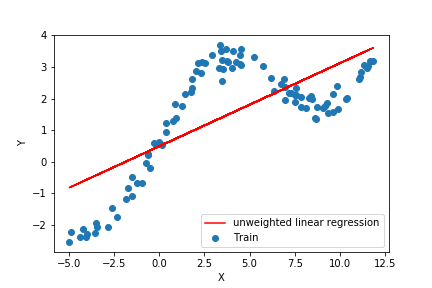
\includegraphics[width=4in,height=2.8in]{2_d1.png} 
    \caption{unweighted linear regression} 
    \label{Fig4}
    \end{figure}

    \textbf{Part d(\romannumeral2):}\\
    \begin{figure}[H]  
    \centering  
    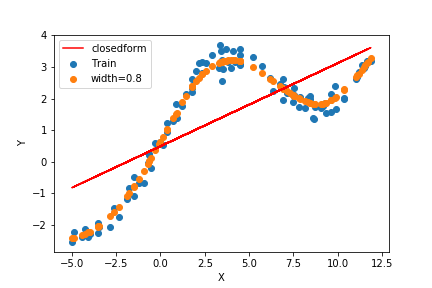
\includegraphics[width=4in,height=2.8in]{2_d2.png} 
    \caption{Locally weighted linear regression with a bandwidth parameter $\tau = 0.8$} 
    \label{Fig5}
    \end{figure}


    \textbf{Part d(\romannumeral3):}\\
    \begin{figure}[H]  
    \centering  
    \includegraphics[width=7.4in,height=6in]{2_d3.png} 
    \caption{unweighted linear regression with different bandwidth parameters} 
    \label{Fig6}
    \end{figure}

    In eq(\ref{eq9}), we note that the weights depend on the particular point $x$ at which we are trying to evaluate $x$. The bandwidth parameter $\tau$ controls how quickly the weight of a training example falls off with distance of its $x^{(i)}$. If $|x - x^{(i)}|$ is large, the weight is small, if $|x - x^{(i)}|$ is small, the weight is close to 1. Hence, if $\tau$ is small, its effect will equal to the large $|x - x^{(i)}|$ which let $\mathbf{w}$ more 'emphasis' on reducing the error at this point. If $\tau$ is large, the weigh is close to 1, which is close to unweighted linear regression. (This explanation is partly inspired by stanford cs229-note1.)
    \begin{equation}
    r^{(i)} = \exp\left(-\frac{(x - x^{(i)})^2}{2{\tau}^2}\right)
    \label{eq9}
    \end{equation}
\end{homeworkProblem}

\begin{homeworkProblem}
    \large Derivation and Proof\\

    \textbf{Solution}

    \textbf{Part a:}\\
    1D case of linear function:
    \begin{equation}
    h(x) = \omega_1x + \omega_0
    \label{eq10}
    \end{equation}

    The sum squared error:

    \begin{equation}
    L = \frac{1}{2}\sum_{i=1}^{N}(y^{(i)} - h(x^{(i)}))^2
    \label{eq11}
    \end{equation}

    From eq(\ref{eq10}) and eq(\ref{eq11}), we can get the partial derivation of L:
    \begin{equation}
    \begin{aligned}
    \frac{\partial L}{\partial \omega_0} &= \frac{\partial{\frac{1}{2}\sum_{i=1}^{N}(y^{(i)} - \omega_1x^{(i)} - \omega_0)^2}}{\partial \omega_0}
    \\
    &= - \sum_{i=1}^{N}(y^{(i)} - \omega_1x^{(i)} - \omega_0)
    \\
    &= N\omega_0 + \omega_1\sum_{i=1}^{N}x^{(i)} - \sum_{i=1}^{N}y^{(i)}
    \\
    &= N(\omega_0 + \omega_1\bar{X} - \bar{Y})
    \\
    \frac{\partial L}{\partial \omega_1} &= \frac{\partial{\frac{1}{2}\sum_{i=1}^{N}(y^{(i)} - \omega_1x^{(i)} - \omega_0)^2}}{\partial \omega_1}
    \\
    &= \sum_{i=1}^{N}x^{(i)}(y^{(i)} - \omega_1x^{(i)} - \omega_0)
    \\
    &= \sum_{i=1}^{N}(x^{(i)}y^{(i)} - \omega_1x^{(i)^2} - \omega_0x^{(i)})
    \\
    &= \sum_{i=1}^{N}(x^{(i)}y^{(i)} - \omega_1x^{(i)^2}) - N\omega_0\bar{X}
    \label{eq12}
    \end{aligned}
    \end{equation}
    where $\bar{X}$ is the mean of $\left\{x^{(1)}, x^{(2)}, \cdots, x^{(N)}\right\}$ and $\bar{Y}$ is the mean of $\left\{y^{(1)}, y^{(2)}, \cdots, y^{(N)}\right\}$. Let the partial derivation of L be equal to zero, respectively, the solution for $\omega_0$ and $\omega_1$ for this 1D case of linear regression is derived as follow:
    \begin{equation}
    \begin{aligned}
    \frac{\partial L}{\partial \omega_0} &= N(\omega_0 + \omega_1\bar{X} - \bar{Y}) = 0
    \\
    \Rightarrow \omega_0 &= \bar{Y} - \omega_1\bar{X}
    \label{eq13}
    \end{aligned}
    \end{equation}

    \begin{equation}
    \begin{aligned}
    \frac{\partial L}{\partial \omega_1} &= \sum_{i=1}^{N}(x^{(i)}y^{(i)} - \omega_1x^{(i)^2}) - N\omega_0\bar{X}
    \\
    &=  \sum_{i=1}^{N}(x^{(i)}y^{(i)} - \omega_1x^{(i)^2}) - N(\bar{Y} - \omega_1\bar{X})\bar{X}
    \\
    &= \sum_{i=1}^{N}(x^{(i)}y^{(i)} - \omega_1x^{(i)^2}) - N\bar{Y}\bar{X} - N\omega_1\bar{X}^2 = 0
    \\
    \Rightarrow \omega_1 &= \frac{\sum_{i=1}^{N}x^{(i)}y^{(i)} - N\bar{Y}\bar{X}}{\sum_{i=1}^{N}x^{(i)^2} - N\bar{X}^2}
    \\
    &= \frac{\frac{1}{N}\sum_{i=1}^{N}x^{(i)}y^{(i)} - \bar{Y}\bar{X}}{\frac{1}{N}\sum_{i=1}^{N}x^{(i)^2} - \bar{X}^2}
    \label{eq14}
    \end{aligned}
    \end{equation}

    \textbf{Part b(\romannumeral1):}\\
    \begin{equation}
    \begin{aligned}
    \mathbf{A} &= \mathbf{U\Lambda U^T} 
    \\
    &=  \sum_{i=1}^{d}\lambda_iu_iu_i^T
    \label{eq15}
    \end{aligned}
    \end{equation}

    \begin{equation}
    \begin{aligned}
    \mathbf{z^TAz} &= \mathbf{z^TU\Lambda U^Tz} 
    \\
    &=  \sum_{i=1}^{d}\lambda_iz^Tu_iu_i^Tz
    \\
    &= \sum_{i=1}^d\lambda_i\Vert u_i^Tz\Vert_2^2, (z \neq 0)  
    \label{eq16}
    \end{aligned}
    \end{equation}

    It is obviously that $\sum_{i=1}^d\lambda_i\Vert u_i^Tz\Vert_2^2 > 0$ iff $\lambda_i > 0$ for each $i$. So, $\mathbf{A}$ is PD iff $\lambda_i > 0$ for each $i$.\\

    \textbf{Part b(\romannumeral2):}\\
    The matrix $\mathbf{\Phi^T\Phi}$ is real and symmetric, so it can be expressed by $\mathbf{\Phi^T\Phi} = \mathbf{U\Lambda U^T}$, so
    \begin{equation}
    \begin{aligned}
    \mathbf{z^T\Phi^T\Phi z} &= \mathbf{z^TU\Lambda U^Tz} 
    \\
    &=  \sum_{i=1}^{d}\lambda_i^2z^Tu_iu_i^Tz
    \\
    &= \sum_{i=1}^d\lambda_i^2\Vert u_i^Tz\Vert_2^2 \geq 0, (z \neq 0)  
    \label{eq16}
    \end{aligned}
    \end{equation}

    \begin{equation}
    \begin{aligned}
    \mathbf{z^T(\Phi^T\Phi + \beta I) z} &= \mathbf{z^TU(\Lambda + \beta) U^Tz} 
    \\
    &=  \sum_{i=1}^{d}(\lambda_i^2 + \beta)z^Tu_iu_i^Tz
    \\
    &= \sum_{i=1}^d(\lambda_i^2 + \beta)\Vert u_i^Tz\Vert_2^2 > 0, (z \neq 0), 
    \\   
    \label{eq16}
    \end{aligned}
    \end{equation}
    because $(\lambda_i^2 + \beta)$ always larger than zero. Hence, for any $\beta > 0$, ridge regression makes the matrix $\mathbf{\Phi^T\Phi + \beta I}$ PD.




\end{homeworkProblem}

\pagebreak

\end{document}